\documentclass{acm_proc_article-sp}
\usepackage[utf8]{inputenc}

\renewcommand{\paragraph}[1]{\vskip 6pt\noindent\textbf{#1 }}
\usepackage{hyperref}
\usepackage{graphicx}
\usepackage{url}

\providecommand{\tightlist}{%
  \setlength{\itemsep}{0pt}\setlength{\parskip}{0pt}}

\title{\$patial: Interactive Tool to Model HDB Resale Prices using
Geographically Weighted Regression}
\subtitle{Guided by Associate Professor of Information Systems: Dr.~Kam Tin Seong}


% Add imagehandling
\usepackage{graphicx}
% Redefine \includegraphics so that, unless explicit options are
% given, the image width will not exceed the width of the page.
% Images get their normal width if they fit onto the page, but
% are scaled down if they would overflow the margins.
\makeatletter
\def\ScaleIfNeeded{%
  \ifdim\Gin@nat@width>\linewidth
    \linewidth
  \else
    \Gin@nat@width
  \fi
}
\makeatother
\let\Oldincludegraphics\includegraphics
{%
 \catcode`\@=11\relax%
 \gdef\includegraphics{\@ifnextchar[{\Oldincludegraphics}{\Oldincludegraphics[width=\ScaleIfNeeded]}}%
}%

\numberofauthors{2}
\author{
\alignauthor Shawn CHUA Jun Yong \\
        \affaddr{School of Information Systems\\
Singapore Management University (SMU)}\\
       \email{\href{mailto:shawn.chua.2018@sis.smu.edu.sg}{\nolinkurl{shawn.chua.2018@sis.smu.edu.sg}}}
\and \alignauthor Olivia GOO Yu Ya \\
        \affaddr{School Of Social Sciences\\
Singapore Management University (SMU)}\\
       \email{\href{mailto:olivia.goo.2018@socsc.smu.edu.sg}{\nolinkurl{olivia.goo.2018@socsc.smu.edu.sg}}}
\and }

\date{}

%Remove copyright shit
\permission{}
\conferenceinfo{} {}
\CopyrightYear{}
\crdata{}

% Pandoc syntax highlighting

% Pandoc citation processing


\begin{document}
\maketitle

\begin{abstract}
Valuing housing prices has seen a surge in popularity over the years
amongst policy planners and economist due to the significant impact that
properties have on the economy and society. The current hedonic pricing
models used in the market fails to take into account the effect of local
spatial features on the housing prices which however there has been
increasing interest and studies carried out on Geographically Weighted
Regression (GWR) model, a more precise regression model to stimulate the
spatial distribution of housing prices. There are several GWR models
available which poses a challenge to casual users who would like to
conduct a simple and understandable analysis of the spatial distribution
of housing prices. Therefore to address this issue, we developed
\$patial, an interactive and accessible application with an user
friendly interface to aid economists and policy planners to effortlessly
explore how variations of spatial features such as number of shopping
malls surrounding the housing estate in different locations affects the
price of the housing flats.
\end{abstract}

\hypertarget{introduction}{%
\section{Introduction}\label{introduction}}

With rapid urbanization and population growth, the demand for housing
around the world is increasing. The volume of housing transactions
globally has seen a boom and global housing markets have been steadily
climbing up the price index (IMF Global Housing Watch, n.d.). Home
ownership being one of the universal signs of success and prosperity due
to it being a long term investment places housing prices as an emerging
subject of interest amongst policy planners, economists and home owners.

The existing hedonic housing pricing models are linear and does not
account for spatial effects on the price of housing flats as such there
is emerging interest in using GWR to accurately model housing prices
(Chin et al., n.d.). In order to solve the current gaps in the existing
pricing models, for the purpose of our project we will be making use of
R Shiny an open-source tool to build user-friendly GWR models for
analysis to show the correlation between spatial attributes and resale
flat prices.

We have selected Singapore's housing market as our case study in this
project as Singapore is known globally as the ``tiny red dot'' with
limited amount of land space thus geographically constrained and albeit
that, there has been an increase in construction of public housing in
Singapore as a result of the rising number of population which makes it
relevant to explore the effects of spatial variations on the housing
prices.

This research paper documents the research and methods used in the
process of implementing the GWR model in our application in relation to
public housing prices. Section 1 provides a general introduction of the
paper and motivations and objectives of the research. Section 2 provides
a review of related papers, section 3 details the review of the
analytical techniques used for visualizing and analyzing data. The
results and future improvements are discussed in section 4 and the paper
is concluded by highlighting the future direction of the research in
section 5.

\hypertarget{review-of-related-work}{%
\section{Review of Related Work}\label{review-of-related-work}}

The development of \$patial is inspired by two published papers.

The first paper being EzModel (Chin et al., n.d.) where two models, GWR
and mixed (semiparametric) GWR is used in the analysis of the datasets
and the second paper being Simple Geo-Spatial Analysis using R-shiny (li
et al., n.d.). The GWR model used in both papers is a local statistical
technique that takes into account the spatial non-stationary objects via
the coefficients obtained from each variable fore each resulting
observation in the regression model. The GWR model used is calibrated in
three steps, firstly a total of five different kernel functions to
calibrate the parameters before running the GWR, the five kernels used
are Gaussian, Exponential, Box-car, Bi-Square and Tri-cube which are
categorized into continuous and discontinuous kernels in order to
determine the allocation of weights to observations. Secondly, fixed and
adaptive weighting scheme which affects the third parameter bandwidth is
calibrated where users are allowed to choose if they would want to make
use of the fixed or adaptive weighting scheme to choose determine the
bandwidth applied to the observations. Lastly, in determining bandwidth,
two other statistical methods- Cross-Validation score and Akaike
Information Criterion is used. EzModel includes a second model in its
paper known as the mixed GWR model which allows for analysis of global
and local variables where the global variables are fixed as independent
variables and the local variables as dependent variables.

\hypertarget{data-collection-data-preparation}{%
\section{Data Collection \& Data
Preparation}\label{data-collection-data-preparation}}

\hypertarget{data-collection}{%
\subsection{Data Collection}\label{data-collection}}

The 2 main types of data used in our application is:\\
1. HDB Flat Resale Prices Data\\
2. Data on features provided to user which is used as independent
variables in the GWR model\\

The fixed spatial features provided by \$patial are:\\
1. Locations of MRT stations\\
2. Primary School Locations\\
3. Secondary School Locations\\
4. Community Centre Locations\\
5. Supermarkets Locations\\
6. Sports Facilities Locations\\
7. Preschools Locations\\
8. Hawkers Locations\\
9. Shopping Malls Locations\\

With the exception of:\\
• Shopping Malls Location -- Wikipedia\\
• MRT and LRT Location -- mytransport.sg\\
The rest of the datasets are obtained from data.gov.sg.

\hypertarget{data-preparation}{%
\subsection{Data Preparation}\label{data-preparation}}

The datasets identified above came in different file types containing
differing data types, some processing must be done for all the imported
data to be integrated into the analysis.

The school dataset we obtained contains all schools ranging from primary
to tertiary education (specifically junior colleges), therefore we
decided to extract data only for primary and secondary schools and keep
them as separate datasets for further analysis. Primary and Secondary
schools are being focused on for the purpose of this study as we felt
that, homeowners will be more concerned for the distance of primary and
secondary schools seeing those that attend them are of the younger age
group and parents may not want them to travel far. For the datasets
containing data on shopping malls and resale flat information, they do
not contain geographical coordinate's data which is needed for our
analysis, therefore we have tapped on the existing Geocode tool provided
by Google Sheets to obtain coordinate data (in longitude and latitude).

After ensuring that all datasets contain coordinate data. We have to
convert those that are in coordinates (longitude and latitude) which are
calculated in degrees into coordinates (X, Y) which are calculated in
meters. This is to ensure proper integration for further analysis when
proximity around resale flats need to be computed and distance metrics
uses distance in meters. Data preparation is mainly done in Rmarkdown
then exported into new csv files for usage in building of Shiny
application.

\hypertarget{methods}{%
\section{Methods}\label{methods}}

The following section reveals the techniques and algorithms used in the
process of designing the application.

\hypertarget{application-architecture}{%
\subsection{Application Architecture}\label{application-architecture}}

The application was developed using Shiny, an R program package. R shiny
is a simple package that is used to build interactive web applications
and dashboards. It runs on a Shiny server hosted by Shinyapps.io , the
datasets mentioned in Section 3.1 are imported and stored in the server.
At the backend, the CSV and Shapefile datasets are cleaned and used for
geocoding, projection and GWR. Whenever the application runs the
datasets are automatically loaded for use. The interactive maps featured
in the application calls on the Leaflet package for it to be
displayed.\\

\begin{figure}[h]
\centering
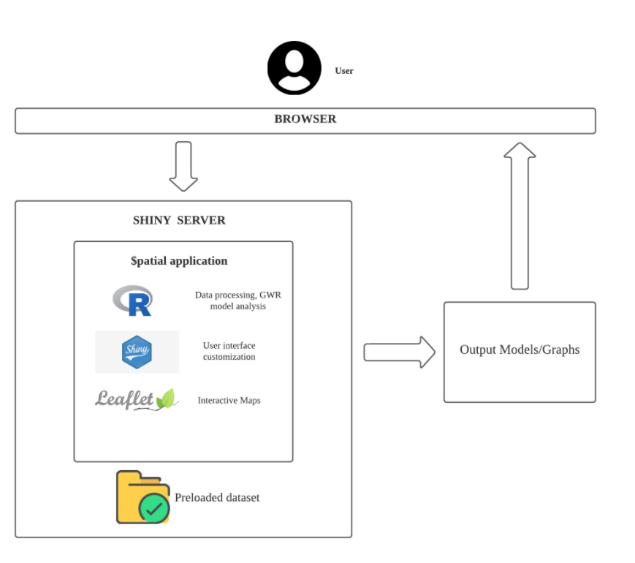
\includegraphics[width=8cm]{App Archite.png}
\caption{Application Architecture Diagram}\label{fig1}
\end{figure}

\hypertarget{application-overview}{%
\subsection{Application Overview}\label{application-overview}}

\hypertarget{r-packages}{%
\subsubsection{R Packages}\label{r-packages}}

The following R Packages are used in the development of the EzModel
Application:\\

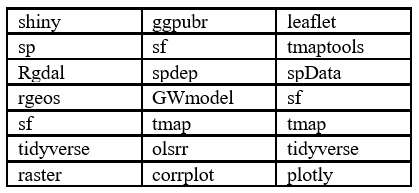
\includegraphics{Table.png}\\

\hypertarget{algorithms}{%
\subsubsection{Algorithms}\label{algorithms}}

4.2.2.1 \textbf{Geographically Weighted Regression}

\$patial makes use of the GWR model, a local statistical technique to
analyze spatial variations in relationships where spatial non-stationary
is assumed and tested by looking at the coefficients of the variables
for each observation in the regression models. The GWR model is based on
the ``First law of Geography'' where everything is related with
everything else, but closer things are more related than remote ones and
the resulting mathematical equation is expressed as such:\\

\begin{figure}[h]
\centering
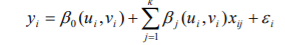
\includegraphics[width=8cm]{Eqn 1.png}
\caption{Application Architecture Diagram}\label{fig2}
\end{figure}

\(y_i\) represents the value of the output variable at the coordinate
location i , \(β_0 (u_i,u_v)\) denotes the coordinates of the i-th point
in space and β\_k (u\_i,u\_v) is a realization of the continuous
functions at point i (Brunsdon et al., 1999). The values used in the
formula depends on the location and surrounding of the observations with
reference to its spatial context. In general, GWR measures the inherent
relationships around each regression point i, each set of regression
coefficient is estimated by weighted least squares (Lu et al., 2014).

The GWR has to be calibrated before it can be used for processing. To
calibrate the formula, firstly we need to distinguish between the
different weighting kernel functions listed below:\\
1. Gaussian\\
2. Exponential~ 3. Box-car\\
4. Bi-square\\
5. Tri-cube\\

\begin{figure}[h]
\centering
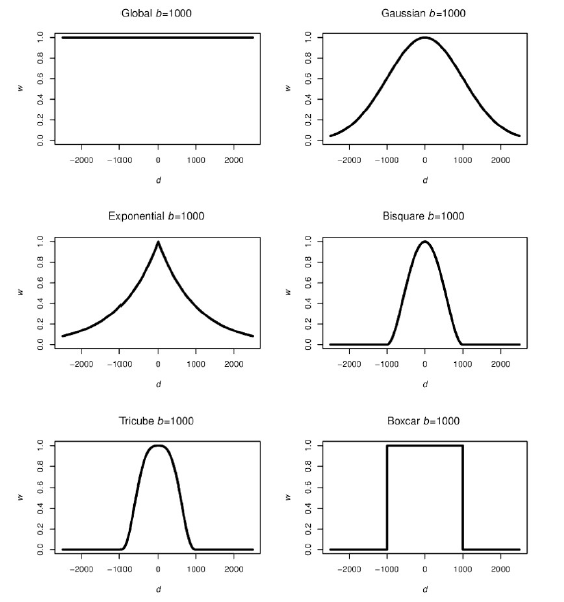
\includegraphics[width=8cm]{function.png}
\caption{Plots showing the different weighting kernel functions}\label{fig3}
\end{figure}

The weighting kernels functions are classified into two categories --
Continuous and Discontinuous kernels. Continuous kernels are Gaussian
and Exponential kernels where the kernels weight all the observations
with a weight that tends towards zero but never produces a zero value
(Bellefon \& Floch, n.d.).\\

\begin{figure}[h]
\centering
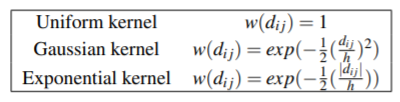
\includegraphics[width=5cm]{continuous.png}
\caption{Formula of Continuous Kernels}\label{fig4}
\end{figure}

The kernels that fall into the discontinuous categories are Box-car,
Bi-square and Tri-cube. The Box-Car kernel handles a continuous
observation in a discontinuous method and Bi-square, Tri-cube kernels
produce observations that are of decreasing weight with increasing
distance however the weight gives a zero value beyond the specified
distance b called bandwidth as seen in figure 5 shown below.\\

\begin{figure}[h]
\centering
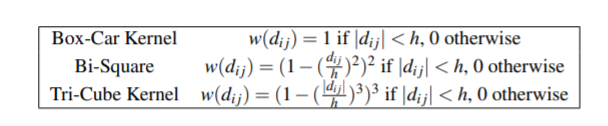
\includegraphics[width=8cm]{discontinuous.png}
\caption{Formula of Discontinuous Kernels}\label{fig5}
\end{figure}

Secondly, there is a need to determine fixed kernel versus adaptive
kernel. Fixed Kernel represents the extent of the kernel that is
determined by the distance to the point of interest which is fixed and
hence the kernel would appear the same at any location (Bellefon \&
Floch, n.d.). Additionally, a fixed kernel causes the regression to vary
significantly as in low-density areas, if the fixed kernel is too small
the number of points that is used in regression would be too little
whereas if the area is dense a fixed kernel that is too large would
overlook the variations in the area. Hence another alternative would be
the adaptive kernel which represents the extent of the kernel that is
determined by the number of neighbors that the point of interest has
which varies according to the bandwidth adjusted according to the
context of the observation in which the bandwidth increases and
decreases following the density of the data points. Lastly, there is a
need to calibrate the choice of bandwidth used in the GWR model as the
bandwidth chosen affects the results produced. Aside from allowing users
to input the pre-defined bandwidth of their choice, there exists two
other statistical methods which can assist in choosing the most suitable
bandwidth. Firstly, the cross-validation criteria given by the formula
as shown in figure 6.\\

\begin{figure}[h]
\centering
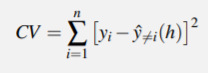
\includegraphics[width=5cm]{cv.png}
\caption{Formula of cross-validation criteria}\label{fig6}
\end{figure}

CV represents the cross-validation score and h represents the bandwidth.
If bandwidth h, minimizes the cross-validation score it is the most
suitable bandwidth value as it maximizes the GWR model's predictive
power (Bellefon \& Floch, n.d.).

Secondly, the adjusted akaike criterion given by the formula as shown in
figure 7.\\

\begin{figure}[h]
\centering
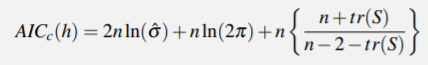
\includegraphics[width=8cm]{aac.png}
\caption{Formula of Adjusted Akaike Criterion}\label{fig7}
\end{figure}

n represents the sample size which and h represents the bandwidth. The
AIC criterion generally prefers larger bandwidth values as compared to
the cross-validation criterion. Therefore, the value of bandwidth
minimizing these two statistical methods is an important indication of
the relevance of Geographically Weighted Regression modelling on the
study area.
\setlength{\parindent}{0in}

\end{document}
